\documentclass[amsfonts, amssymb, prl, superscriptaddress, notitlepage, twocolumn, nofootinbib]{revtex4-2}

\usepackage{amsmath}    
\usepackage{graphicx}   
\usepackage{verbatim}   
\usepackage{color}      
\usepackage{hyperref}   
%\usepackage{subcaption}
\usepackage[english]{babel}
\usepackage{ucs}
\usepackage[utf8x]{inputenc}
\usepackage{subfigure}
\usepackage[autostyle]{csquotes}
%\MakeOuterQuote{"}
\usepackage{float}
\usepackage{textcomp}
\usepackage{xspace}
\usepackage{orcidlink}

\newcommand{\Corr}{\operatorname{Corr}}
\newcommand{\Cov}{\operatorname{Cov}}
\DeclareMathOperator{\E}{\mathbb{E}} 
\DeclareMathOperator{\Var}{Var}
\newcommand{\bc}[2]{$\beta$#1cell#2}
\newcommand{\lra}[1]{\langle{}#1\rangle}
\newcommand{\Ca}{Ca$^{2+}$\xspace}
\newcommand{\Cac}{[Ca${}^{2+}$]$_{\rm{c}}$\xspace}


\begin{document}

\title{Two cultures}
\author{L.~Kopitar \orcidlink{0000-0002-6647-9988}}
\affiliation{University of Maribor, Slovenia}

\author{M.~Tancer Verboten}
\affiliation{University of Maribor, Slovenia}

\author{G.~Štiglic \orcidlink{0000-0002-0183-8679}}
\affiliation{University of Maribor, Slovenia}

\author{R.~Watson \orcidlink{0000-0001-8040-7625}}
\affiliation{Southwest Medical University, China }

\author{D.~Korošak \orcidlink{0000-0003-3818-1233} }
\thanks{Corresponding author:\\dean.korosak@um.si}
\affiliation{University of Maribor, Slovenia}
%\affiliation{University of Maribor, Faculty of Civil Engineering, Transportation Engineering and Architecture, Maribor, Slovenia}
% https://orcid.org/0000-0003-3818-1233





\date{\today}

\begin{abstract}
The evaluation of university performance has traditionally relied heavily on research output, with academic journal publications playing a central role. However, the reliance on publication metrics such as total citations, journal impact factors, and h-indices to assess both institutions and individual academics has been fraught with controversy. Initiatives like DORA and CoARA have emerged to mitigate the potential misuse of these metrics, advocating for a more qualitative approach to research assessment that includes aspects of research culture, inclusivity, and diversity. Our study explores how academic journal publications are utilized across universities and countries, and whether the adherence to declarations such as DORA and CoARA influences this utilization. The analysis, conducted using the OpenAlex API, focused on universities ranked in the CWTS Open Ranking, using the ratio of publications in MDPI versus the Big Five publishers as a measure of publishing habits. Results indicated significant differences in publishing practices, with a clear separation into two distinct scholarly publishing cultures. The MDPI ratio distributions revealed a difference both at the university and country levels, highlighting an increasing gap between new and old EU member states. Furthermore, the study demonstrated a correlation between a university's rank and its publishing culture, as well as between national innovation potential, corruption perception, and publishing practices. We argue that...
\end{abstract}

\maketitle 

\section{Introduction}
One of the mainstays of evaluating the performance of universities is their performance in research, and a major plank of that evaluation is constituted by publication in academic journals. Likewise, the evaluation of individual academics follows similar processes. 
We have previously discussed the controversies involved in using publication in academic journals to evaluate individual academics~\cite{watson2023assessing} and many of those issues apply to the use of publication in academic journals apply to the evaluation of universities. Specifically, the use of publication metrics such as total citations to articles, impact factor of journals and h-indices of individual academics. 
To mitigate the use or inappropriate use of publication metrics there have been initiatives such as DORA (San Francisco Declaration on Research Assessment) and, more specific to European universities, CoARA (Coalition for Advancing Research Assessment, Barcelona declaration). Both of these declarations eschew the use of raw bibliometrics. DORA approaches this by urging signatories to avoid the use of journal impact factors and to consider, for example, narrative CVs, and CoARA provides for more qualitative indicators of research quality, urging signatories to consider aspects of research culture such as inclusivity and diversity. 
Two questions arise. First, how is publication in academic journals used across universities and countries (in Europe/internationally)? Second, is there a difference in the use if publication in academic journals to evaluate research between universities that sign declarations such as DORA and CoARA? 

Towards that end, we used CTWS Open Ranking data for universities listed there making comparisons on the basis of total publications, type of publication and publishers used. In addition, we analysed open access publishing and retractions to see if patterns could be established and inferences drawn.

In one study~\cite{baccini2019citation} the authors examine how the introduction of bibliometric evaluations in Italy in 2011 led researchers to change their behavior, focusing more on self-citations and strategic citations to improve their evaluation scores. One way to understand such a shift is to use a simple coordination game framework, where the new policy incentivizes researchers to prioritize self-promotion over traditional, cooperative citation practices. This collective shift in behavior demonstrates how policy changes can significantly influence academic norms, leading to a new equilibrium where citation gaming becomes the dominant strategy to achieve career advancements.

In many scientific fields, research funding affects publication and productivity. Grant funding generally increases publication output and impact, but this depends on the field of study, researcher experience, and funding mechanism. A systematic review of comparative studies found that awarded applicants published 0.14 articles per year more than rejected applicants~\cite{saygitov2018impact}. Recently, detailed grant application data analysis have found larger positive effects of funding on publication outcomes. A multi-year Norwegian research grant study found that recipients publish 5.14 more articles than the control group~\cite{adda2023impact}. The same study found substantial positive effects on publication quality metrics, including an increase in publications weighted by journal influence score and in citation-weighted publications. An analysis of Swiss National Science Foundation grants similarly found that funded researchers publish about one additional peer-reviewed article per year in the three years following funding compared to unsuccessful applicants. These additional publications also tend to be more influential as measured by citation counts ~\cite{ heyard2021value}. Funding appears to affect more than just publication numbers. Funded research has higher citation metrics and altmetrics scores, suggesting that grants improve research quality and dissemination~\cite{heyard2021value}. Importantly, funding affects more than just core project publications. A biomedical research funding study found significant "ripple effects," with even higher increase in publications for papers related to funding, but without principal investigators ~\cite{sattari2022ripple}. This suggests that funding affects research teams and collaborations beyond the funded project. Overall, the evidence indicates that competitive research funding plays an important role in facilitating knowledge creation and dissemination across scientific fields. However, most of the research mentioned above focuses on local or grant funding, while in our study, we aim to capture the trends on a wider scale by comparing the publication trends between different countries or groups of countries.

current scholarly publishing culture shows instability, tipping points, bifurcation into two cultures....

\section{Methods and results}
OpenAlex~\cite{priem2022openalex} is an open-access platform designed to index scientific publications. It provides access to metadata about scientific papers, journals, authors, and ultimately institutions. The OpenAlex API was utilized for simplified and automatized access to data in the OpenAlex repository. The OpenAlex API is freely available and does not necessitate an API key for utilization, making it fairly easy to use. Due to the rate limits, which are implemented to prevent abuse and ensure fair usage, we had to send requests in 30 second intervals. 

We analyzed publishing data for all universities that were ranked in CTWS Open Ranking~\cite{cwts2024leiden}. For each institution, we fetched its data based on ROR ID~\cite{ROR} and publication year. This dataset was then further processed by considering the publication type and calculating the total number of publications. By aggregating ROR ID, year, and journal type, we derived new features such as the number of publications published with MDPI, Taylor\&Francis, Springer Nature, Wiley, Sage, and Elsevier, the number of retracted publications, the number of open access publications, and the number of gold open access publications. These features can be used to examine various indicators of publishing habits and serve as a starting point for comparing institutions publishing culture. 

Here we focus on the ratio, $\rho$, between the number of publications published with MDPI and the Big Five (Springer Nature, Wiley, Elsevier, Taylor\&Francis, Sage) in a given year defined as: 

\begin{equation}
\rho = \frac{N_{\text{MDPI}}}{N_{\text{Big Five}}+N_{\text{MDPI}}}
\end{equation}

where $N_{\text{MDPI}}$ is the number of publications published with MDPI and $N_{\text{Big Five}}$ is the number of publications published with the Big Five publishers.

\begin{figure}
\centering
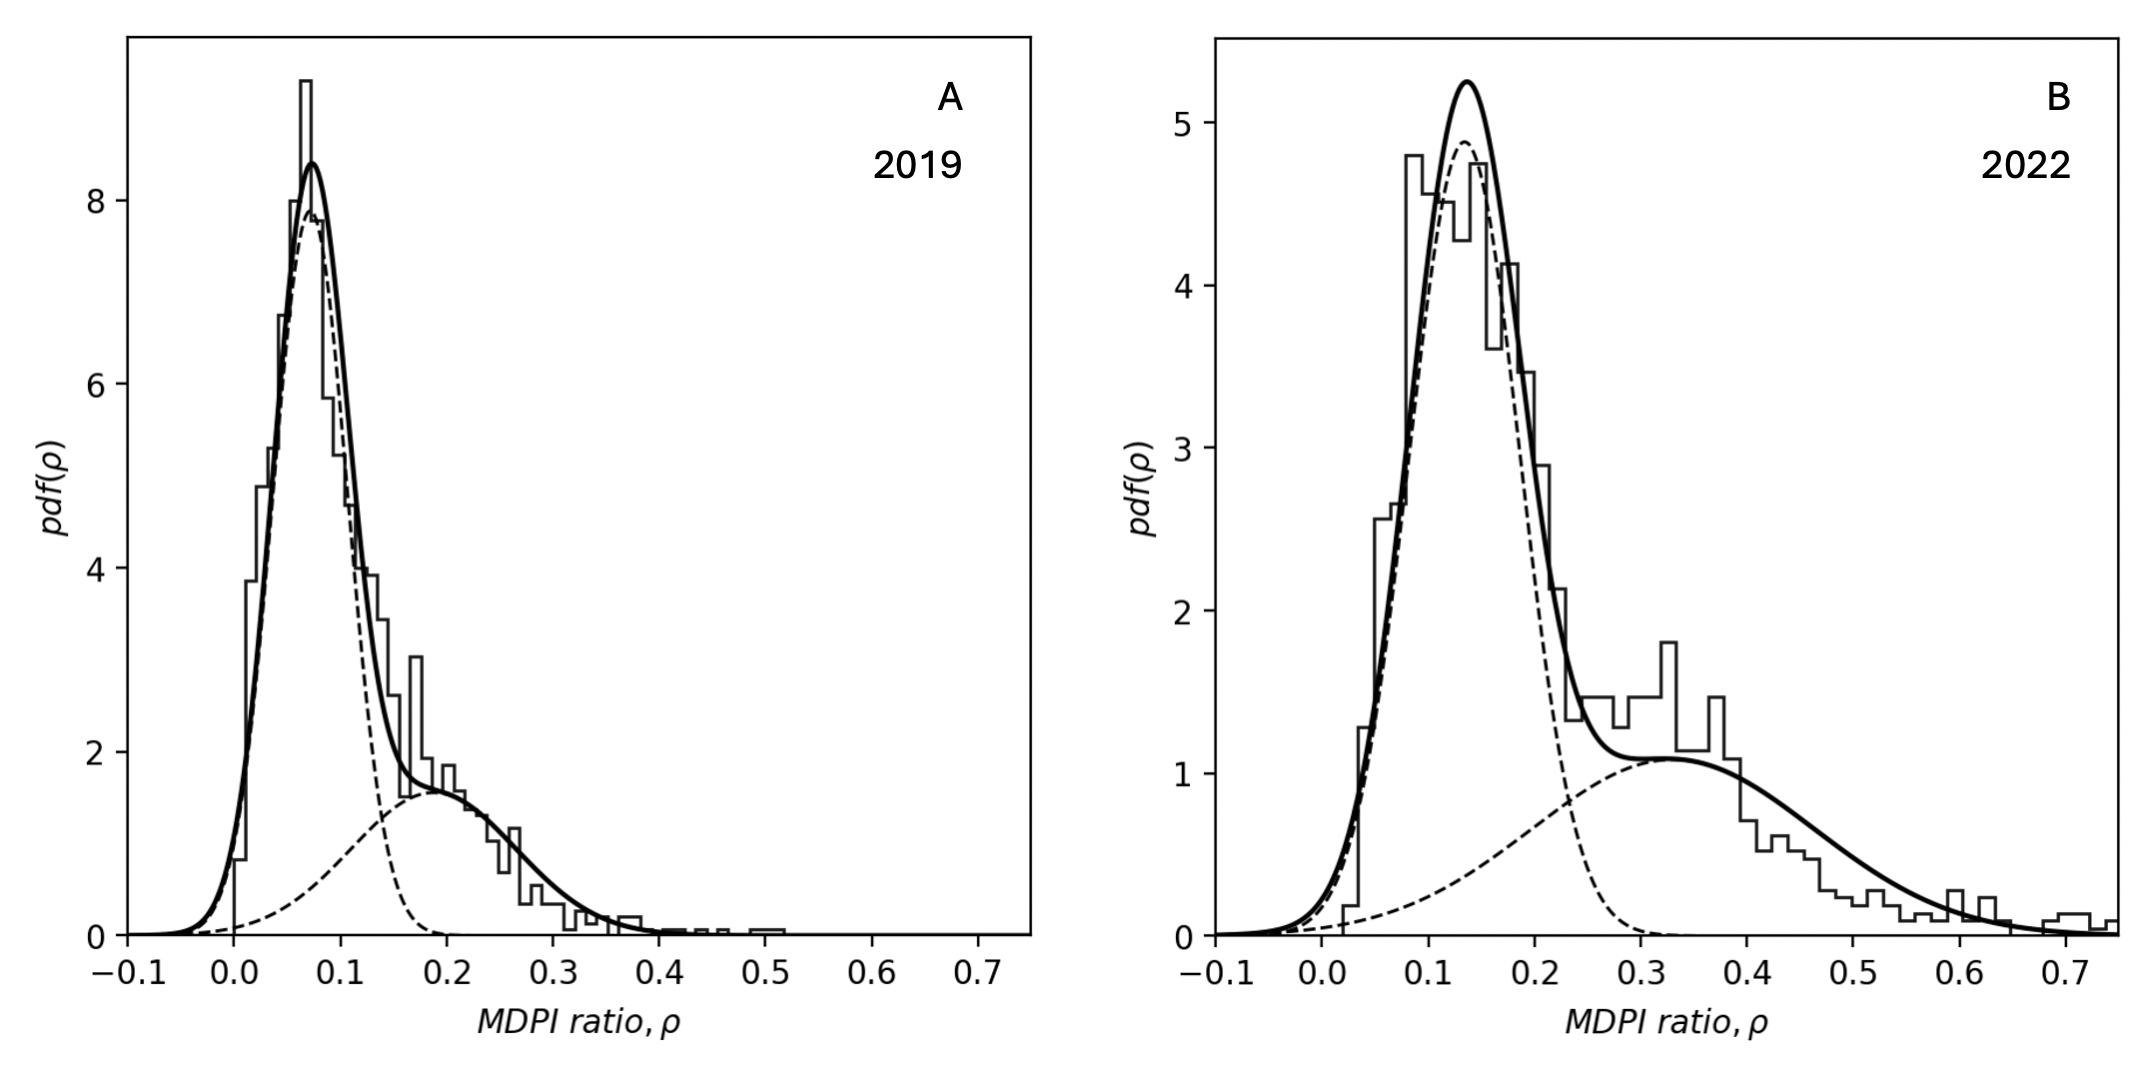
\includegraphics[width=1.0\linewidth]{Fig01.png}
\caption{\label{fig:fig1} {\bf Figure title.} MDPI ratio distributions, university level  
}
\end{figure}

In figure 1 we show the MDPI ratio distribution with universities ranked in CWTS Leiden Open Ranking. The distribution is well described by two-gaussian mixture (full line, individual gaussians  are plotted with dashed lines) and the evolution of the distribution between 2019 (panel A) and 2022 (panel B) clearly shows the separation of means of the two gaussians in the mixture with time.  

\begin{figure}
    \centering
    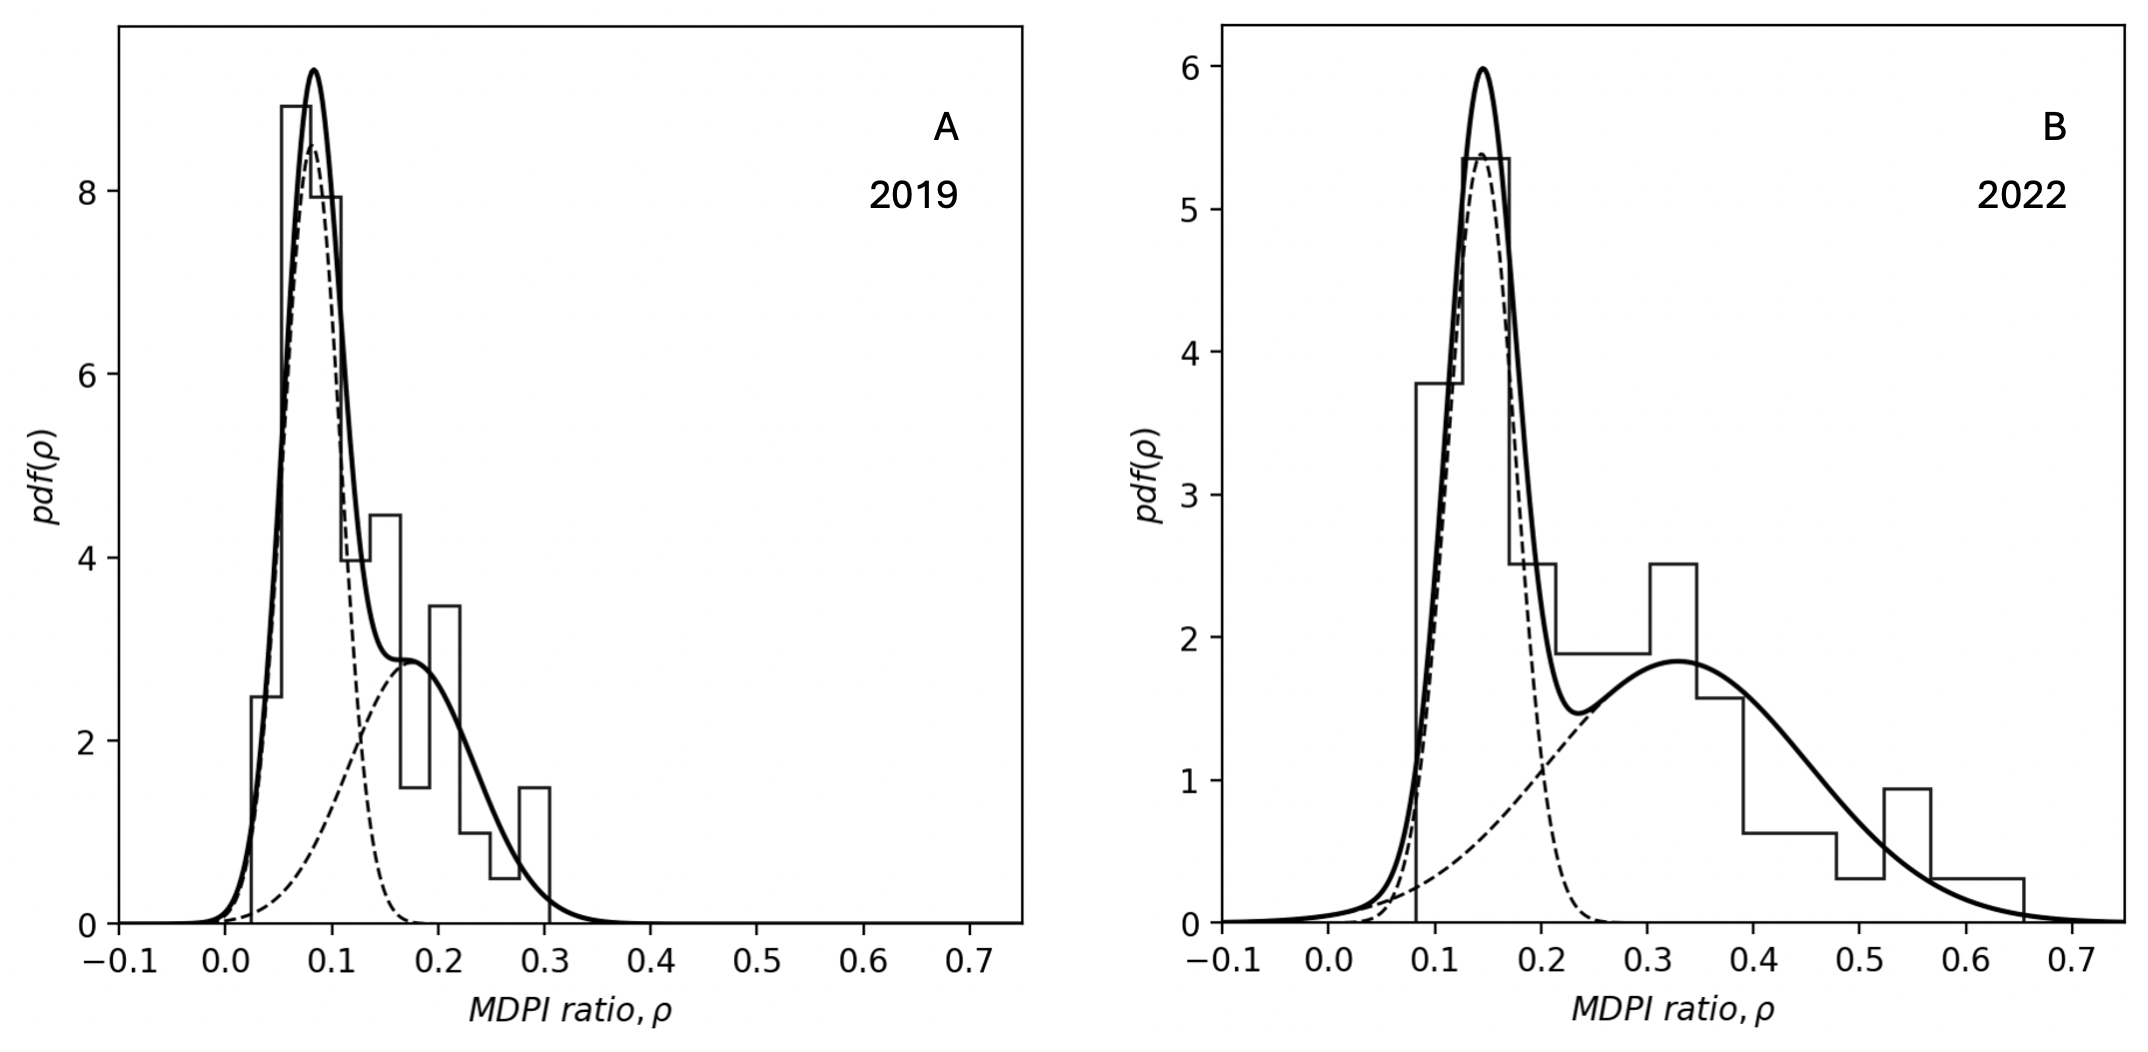
\includegraphics[width=1.0\linewidth]{Fig02.png}
    \caption{\label{fig:fig2} {\bf Figure title.} MDPI ratio distributions, country level  
    }
\end{figure}

In figure 2 we show the MDPI ratio distribution across countries with universities ranked in CWTS Leiden Open Ranking. The distribution is well described by two-gaussian mixture (full line, individual gaussians  are plotted with dashed lines) and the evolution of the distribution between 2019 (panel A) and 2022 (panel B) clearly shows the separation of means of the two gaussians in the mixture with time.  

\begin{figure}
    \centering
    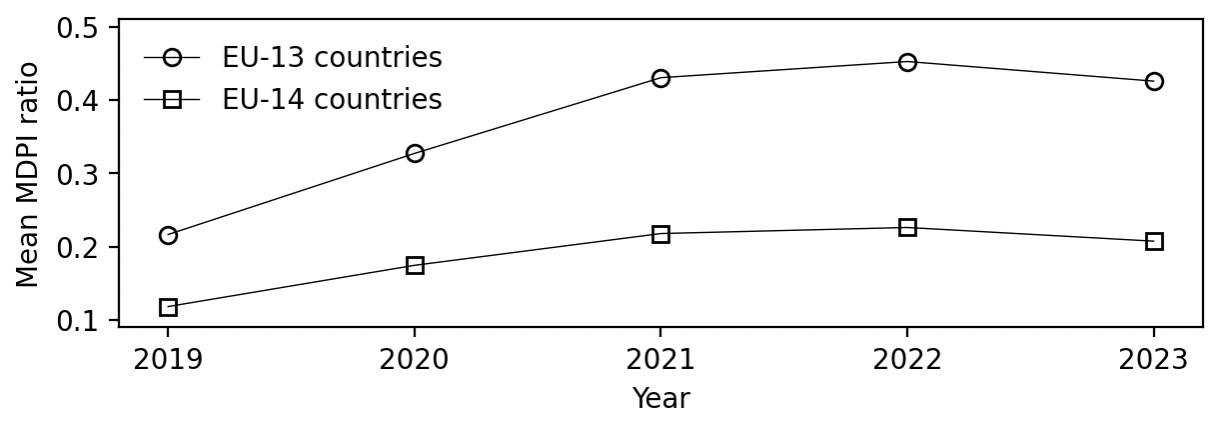
\includegraphics[width=1.0\linewidth]{Fig01a.png}
    \caption{\label{fig:fig3} {\bf Figure title.} Mean MDPI ration vs years for EU-13 and EU-14 countries.  
}
\end{figure}
% EU-14 group = [Austria, Belgium, Denmark, Finland, France, Germany, Greece, Ireland, Italy, Luxembourg, Netherlands, Portugal, Spain, Sweden]
% EU-13 group = [Croatia, Cyprus, Czech Republic, Estonia, Hungary, Lithuania, Poland, Romania, Slovakia, Slovenia]

In figure 3 we show the mean MDPI ratio separately for EU-13 and EU-14 countries, so-called new and old EU member states. The
gap and the increasing trend of the gap over the years in mean MDPI ratio between these two country groups is clearly visible. 

\begin{figure}
    \centering
    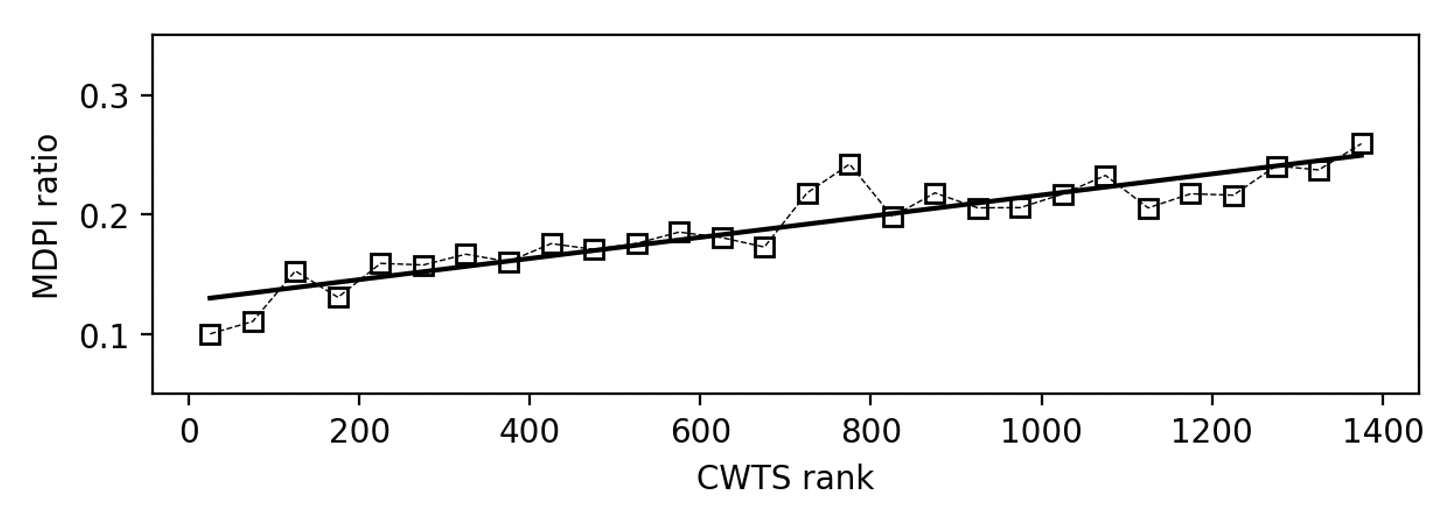
\includegraphics[width=1.0\linewidth]{Fig03.png}
    \caption{\label{fig:fig3} {\bf Figure title.} MDPI ratio vs rank  
}
\end{figure}

In figure 4 we display the relationship between the MDPI ratio and the rank of universities included in CWTS Leiden Open Ranking table. The individual data points in the figure are the averages of MDPI ratios of universities in bins each 50 ranks wide. This relationship can be well described by a simple linear relationship between the rank of the university and its scholarly publishing culture.  

\begin{figure}
    \centering
    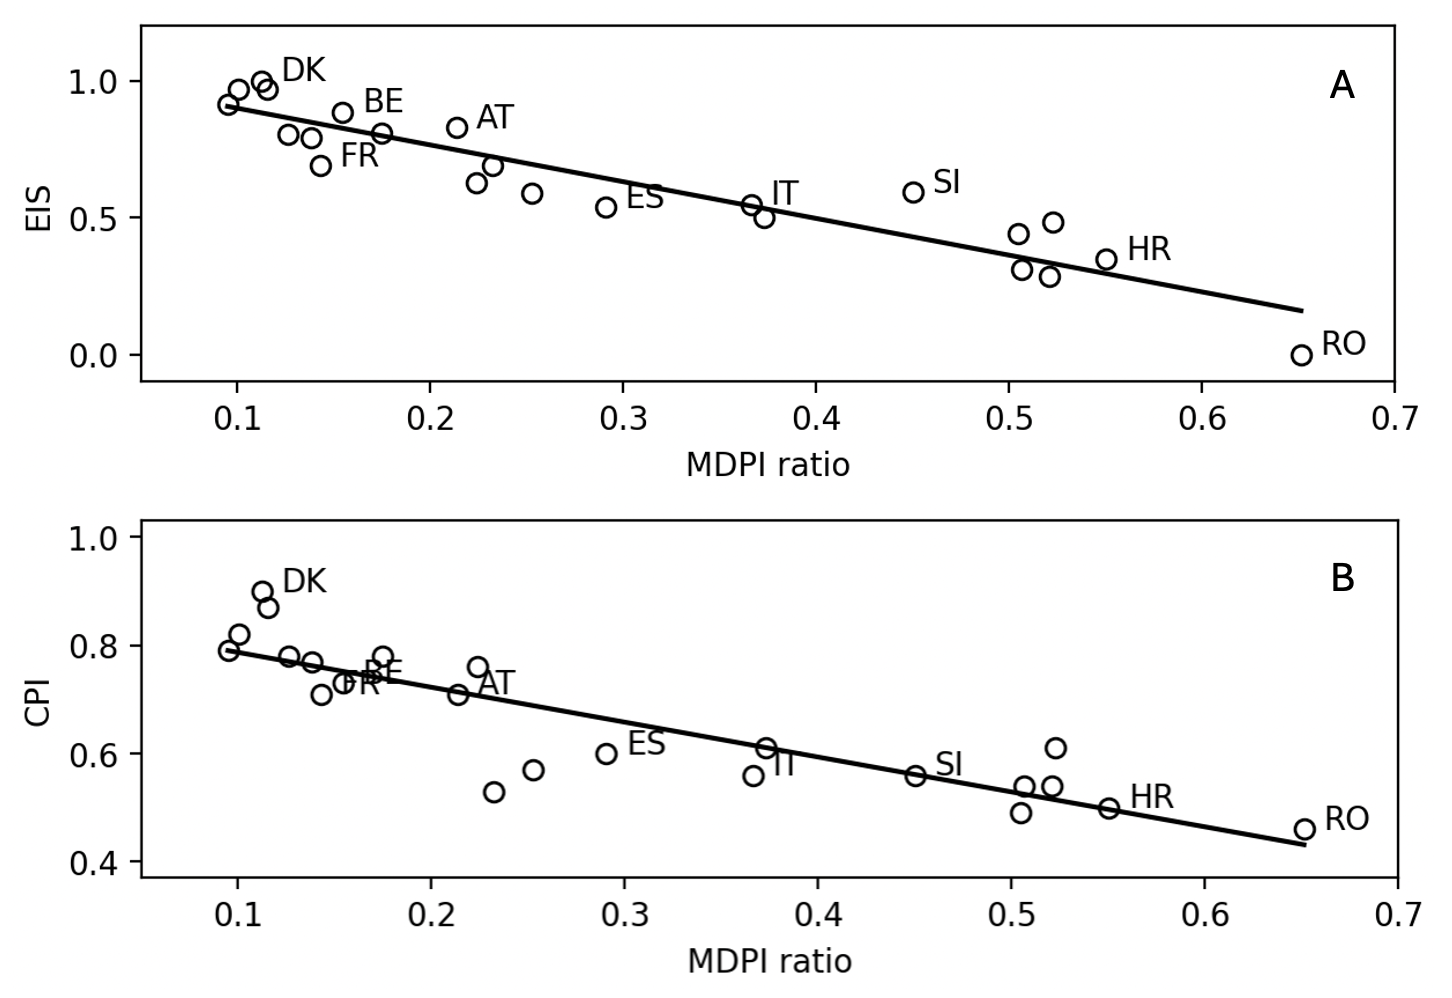
\includegraphics[width=1.0\linewidth]{Fig04.png}
    \caption{\label{fig:fig4} {\bf Figure title.} Innovation potential, corruption perception and scholarly publishing culture  
}
\end{figure}

Figure 5 shows the relationship between innovation potential (EIS), corruption perception (CPI) and the scholarly publishing culture as quantified here through MDPI ratio (panels A and B) on a country level. For clarity only some of countries are indicated with country codes.

\begin{figure}
    \centering
    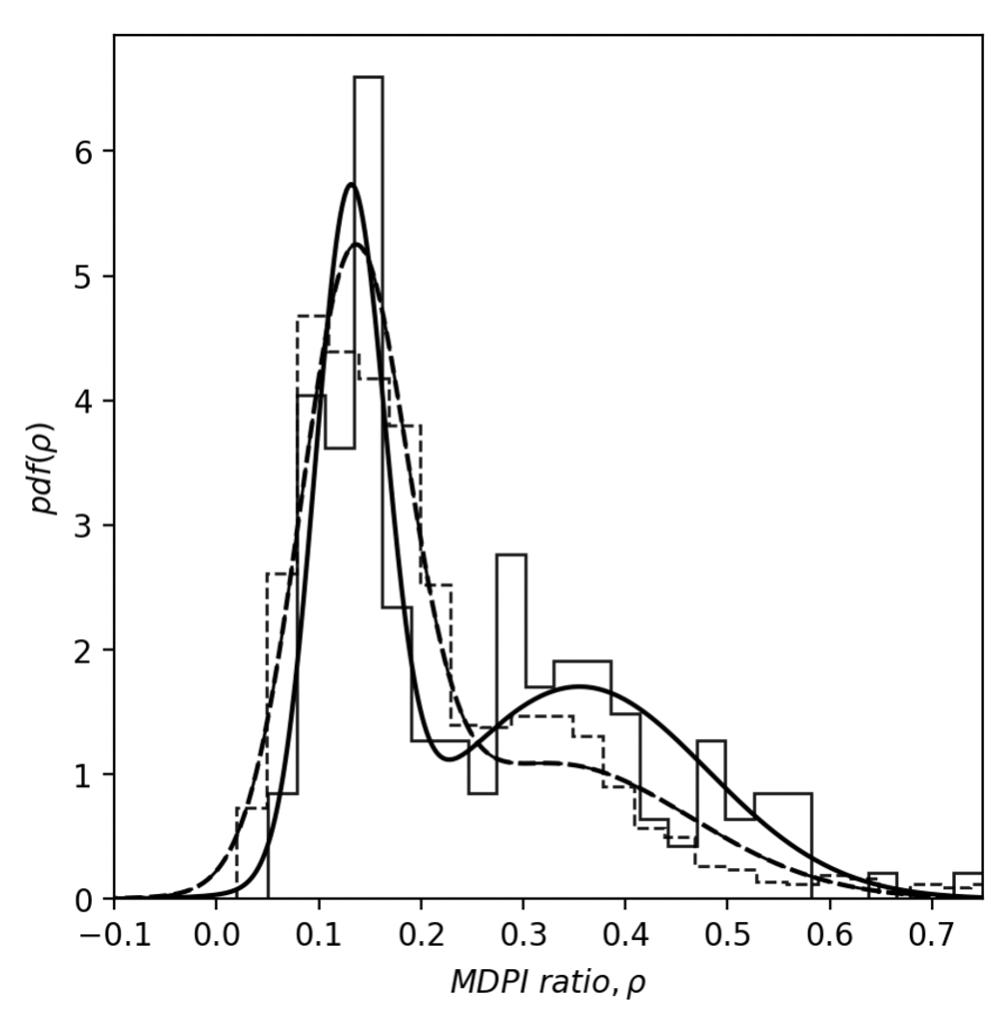
\includegraphics[width=.6\linewidth]{Fig05.png}
    \caption{\label{fig:fig5} {\bf Figure title.} MDPI ratio distributions, CoARA universities  
}
\end{figure}

Figure 6 displays the distribution of MDPI ratio for CoARA universities included in CWTS ranking compared to all CWTS ranked universities. Both distributions are quite similar, exhibiting two-gaussian mixture shape. This puts CoARA group universities in a unique position where one can observe whether in the following years the shift towards more homogeneous publishing practice will happen driven by coalitions tenets.   

\section{Evolution of two cultures in scholarly publishing }
We showed that the MDPI ratio distribution is well described by two-gaussian mixed distribution which is a weighted sum of two gaussian distributions $P(x) = \omega\mathcal{N}(x|\mu_1, \sigma_1) + (1-\omega)\mathcal{N}(x|\mu_2, \sigma_2)$ peaked around mean values $\mu_1, \mu_2$ for MDPI ratios with widths $\sigma_1, \sigma_2$ for EU-14 and EU-13 countries. Suppose that means and variances evolve with time much slower than the values of the weight $0\ge\omega\le 1$.  Therefore, the shape of $P(x)$ will be mostly determined by the time evolution of $\omega$. The emergence of two cultures in scholarly publishing when $\omega > 0$ or when the second peak with $\mu_2 >\mu_1$ occurs.  

To show how two distinct cultures can emerge from a single culture within the realm of scholarly publishing in the EU, we use a coordination game approach. The game involves researchers choosing between two strategies: publishing in established, legacy journals with typically slow reviewing processes (strategy C, cooperate) or in new, fast-reviewing, open-access journals (strategy D, defect). Initially, most researchers follow strategy C, reflecting the traditional approach. However, an increasing push for open science and the appeal of rapid dissemination create incentives for adopting strategy D. Researchers payoffs depend on coordination with peers; higher payoffs are achieved when researchers align with others publishing strategies due to shared benefits like citation practices, visibility, and academic recognition.  

 Let's illustrate this with a simple example. Consider the following form of a coordination game as an example: 
 \begin{table}[H]
\centering
\begin{tabular}{c|cc}
    & \textbf{C} & \textbf{D} \\ \hline
    \textbf{C} & 3,3 & 0,2 \\ 
    \textbf{D} & 2,0 & 1,1 \\ 
\end{tabular}
\end{table}

 If both researchers choose C, they each receive a payoff of 3, showing mutual high benefit from traditional publishing. If one researcher chooses C while the other chooses D, the researcher sticking with C receives 0, while the one choosing D gets 2, reflecting a situation where the traditionalist gains nothing due to a lack of coordination, but the open-access researcher still benefits from the faster dissemination. If both researchers choose D, they each receive a payoff of 1, indicating a lower but shared benefit from mutual participation in the open-access model. With this game we wished to emphasize the benefits of coordinated strategies, with the highest rewards for mutual adherence to traditional methods, and the increasing appeal of open-access publishing despite the challenges of misalignment.

This game has two Nash equilibria: (C,C) and (D,D). Let $x$ be the fraction of players that choose strategy C and $1-x$ fraction of players choosing strategy D. The evolution of a strategy depends on the deviation of players' strategy payoff from the average payoff usually expressed as a replicator equation: $dx/dt = x(\Pi_C-\Pi)$. These are given as:
% equation array for populations
\begin{eqnarray}
    \Pi_C = 3x + 0(1-x) = 3x \\
    \Pi_D = 2x + (1-x) = 1+x \\
    \Pi = x\Pi_C + (1-x)\Pi_D.
\end{eqnarray}
In a steady state we have $x(\Pi_C-\Pi)=x(1-x)(\Pi_C-\Pi_D)=x(1-x)(2x-1)=0$ and corresponding fixed points are: $x_+=1$, $x_-=0$ (stable) and $x_* = 1/2$ (unstable). The $x_+$ fixed point corresponds to the single (traditional) publishing culture, so the weight in the two-gaussian mixed model is given by the fraction of cooperators in the population $\omega=x$. 

Introducing mutations, analogous to the variability in publishing strategies, adds complexity to this system. As the mutation rate increases, the fixed points, and thus $\omega$ shift, potentially leading to new equilibria or emergence of the second gaussian peak in P(x). Using the replicator-mutator equation framework we can examine how publishing strategies evolve over time, influenced by replication (where successful strategies proliferate) and mutation (where strategies change randomly). 

Let $q$ and $\lambda$ denote multiplicative and additive mutations as introduced in \cite{mobilia2010oscillatory} and \cite{mittal2020evolutionary}. Additive mutations model experiments with open-access publishing regardless of the current popularity. Over time, if these experiments prove beneficial, the academic community slowly shifts towards open-access. The multiplicative mutations represent a more responsive scholarly community where the success of open-access publishing quickly attracts more scholars. As more scholars see the benefits and switch, the movement towards open-access publishing accelerates. The replicator-mutator equation is given by:
\begin{equation}
    \frac{dx}{dt} = qx\Pi_C+(1-q)(1-x)\Pi_D-x\Pi-\lambda(2x-1)
\end{equation}

Here, we consider two cases of multiplicative mutations parameter: $q=1$ and $q=1/2$. The former is a case with no multiplicative and only additive mutations, the latter combines flip coin style multiplicative mutations with additive mutation. 

With $q=1$ or no multiplicative mutation, we have:
\begin{equation}
    \frac{dx}{dt} = (1-2x)(x^2-x+\lambda)
\end{equation}
The stable points to which the solutions tend are: $x_*=1/2$, $x_{\pm}=(1\pm\sqrt{1-4\lambda})/2$. For small $\lambda$ the steady state fixed points or the weight of the second gaussian peak in the mixed distribution is $x_- =1-\omega=\lambda$.

Let now set $q=1/2$ and allow $\lambda$ to assume negative values $\lambda = -\tilde{\lambda},\, \tilde{\lambda}>0$. The replicator-mutator equation is in this case:
\begin{equation}
    \frac{dx}{dt} = (1-2x)\left(x^2-\tilde{\lambda} +\frac{1}{2}\right).
\end{equation}
One of the fixed points is again at $x_*=1/2$, but the solution for fraction of cooperators choosing C is now $x_+ = \sqrt{\tilde{\lambda}-1/2}$ for $\tilde\lambda\in [3/4,3/2]$ so that $x_+ \in [1/2,1]$. This shows that in this case the stable fixed point (C,C) can, at a bifurcation point where $\tilde\lambda$ crosses a critical point, merge with an unstable fixed point, where even small deviations can push the community towards one of the extremes: either predominantly quality-focused or predominantly quantity-focused publishing. 


\section{Discussion}
The findings of this study reveal significant insights into the current state and evolving trends of scholarly publishing practices among universities and EU countries. The analysis of the MDPI ratio, representing the proportion of publications in MDPI compared to the Big Five publishers, highlights a clear bifurcation in publishing cultures. This separation, evident at both the university and country levels, indicates a growing divergence in publication strategies, influenced by factors such as policy changes and institutional rankings. The increasing gap between EU-13 and EU-14 countries underscores the impact of regional dynamics on academic publishing. Additionally, the correlation between publishing practices and factors like innovation potential and corruption perception suggests that broader socio-economic contexts play a role in shaping research outputs. 

Labor law, universities and research assessment systems across EU: north-west vs south-east comparison 
Response of countries to open access/science EU initiative and the NW-SE divide... EU-13 vs EU-14 gap, ERA harmonization

Open science (REF2029, ...)
  
\begin{center}
--\,--\,--\,--\,--
\end{center}
\vspace{1mm}
\noindent\textbf{Acknowledgements.} DK received financial support from the Slovenian Research Agency (the research core funding program P3-0396 and the research project no.J7-3156). 


\noindent\textbf{Author contributions.} All authors contributed substantially to all aspects of the study.

\noindent\textbf{Conflict of interest.} The authors declare no conflict of interest, financial or otherwise.


\bibliography{refs}{}
\bibliographystyle{apsrev4-1}


\end{document}